\section{Architecture}
\label{architecture}

%generall description about the technologies used in the project and how they interact, also why I used the technologies (advantages and disadvantages); also insert figures of the app and throughout this chapter more of each specific activity
As mentioned above, we decided to implement an Android application for mobile phones. Since the Chrome browser offers an interface for using Bluetooth LE on the web, we decided to develop a Chrome extension to utilize their Web Bluetooth API. \cite{WebBTAPI}

With the extension, we inject a button on the website. The button is used to establish a Bluetooth LE connection between application and extension. Upon successful pairing, the extension is allowed to read characteristics that are advertised from the app. The characteristics contain username and password, which the extension inserts directly into the login fields of the website.

\noindent Before starting with the implementation we defined minimal requirements of the Android application and the Chrome extension: \\

\noindent Minimal requirements of application:
\begin{itemize}
\item Safe storage of credentials
\item Adding, changing and deleting credentials
\item En- and decryption of data 
\item Authentication through biometric identification
\item Establishing a Bluetooth connection with the web extension
\end{itemize}
\vspace{0.3cm}
\noindent Minimal requirements of extension:
\begin{itemize}
\item Injection of a button onto the website
\item Establishment of Bluetooth LE Connection
\item Reading the advertised characteristics
\item Filling credentials into the proper login fields
\end{itemize}


%technical details:
\noindent For convenience purposes, we implemented the application for API level 23 minimum and up using Android Studio as the IDE. To go more into detail about the app, it consists of a main activity \ref{fig:mainactivity}, which contains four different menu items: \textit{Accounts}, which provides the user with an interface to manage their login accounts; \textit{Connection}, where users can establish the Bluetooth connection to send login data to the web browser; \textit{Settings} and \textit{About}. We will go more into detail about the functionality of the activities \textit{Accounts} and \textit{Connection}. Subsequently, we will examine how the application handles data storage, encryption, and authentication in greater detail.

\begin{figure}[H]
\centering
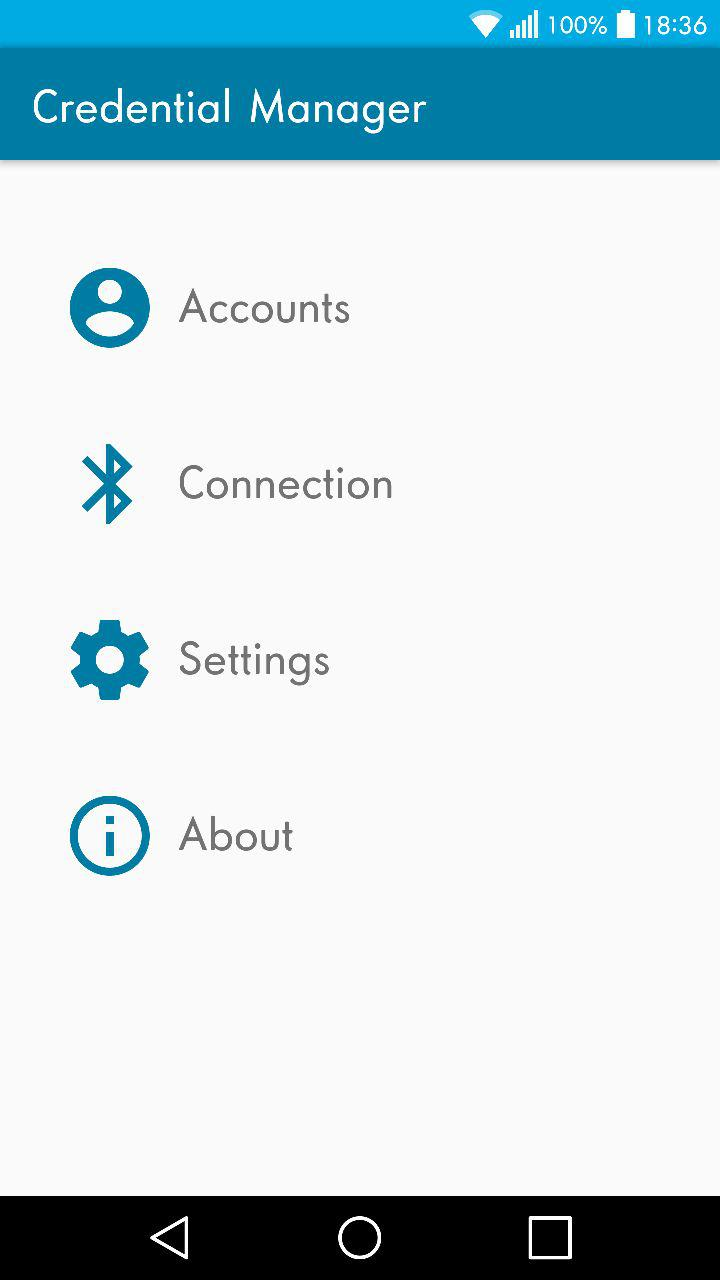
\includegraphics[width=5cm]{images/MainActivity}
\caption[Main activity]{Main activity, which is shown at start up of the app}
\label{fig:mainactivity}
\end{figure}

%-------------------------------------------------------------------------------------

\subsection{Activity for managing Accounts}
By clicking on the menu item \textit{Accounts}, the user is asked to authenticate themselves (Figure \ref{fig:authentication}\protect\subref{auth_screen}). Upon successful verification, the interface in Figure \ref{fig:accountactivity}\protect\subref{show_acc} is shown. The user has an overview of his saved credentials. By clicking the button on the bottom right corner, the activity is switched to Figure \ref{fig:accountactivity}\protect\subref{add_acc}. Here the user can add a new login accounts. Clicking the \texttt{save}-button encrypts and adds the credential to the database.

When clicked on one of the existing credentials in the list, it takes the user to the interface shown in Figure \ref{fig:accountactivity}\protect\subref{change_acc}.  Here data can be changed and saved again. Also, the account can be deleted from the database. When deleting a credential, the user is asked via prompt as seen in Figure \ref{fig:accountactivity}\protect\subref{prompt_delete}.

\begin{figure}[H]
\centering
\subfloat[]{{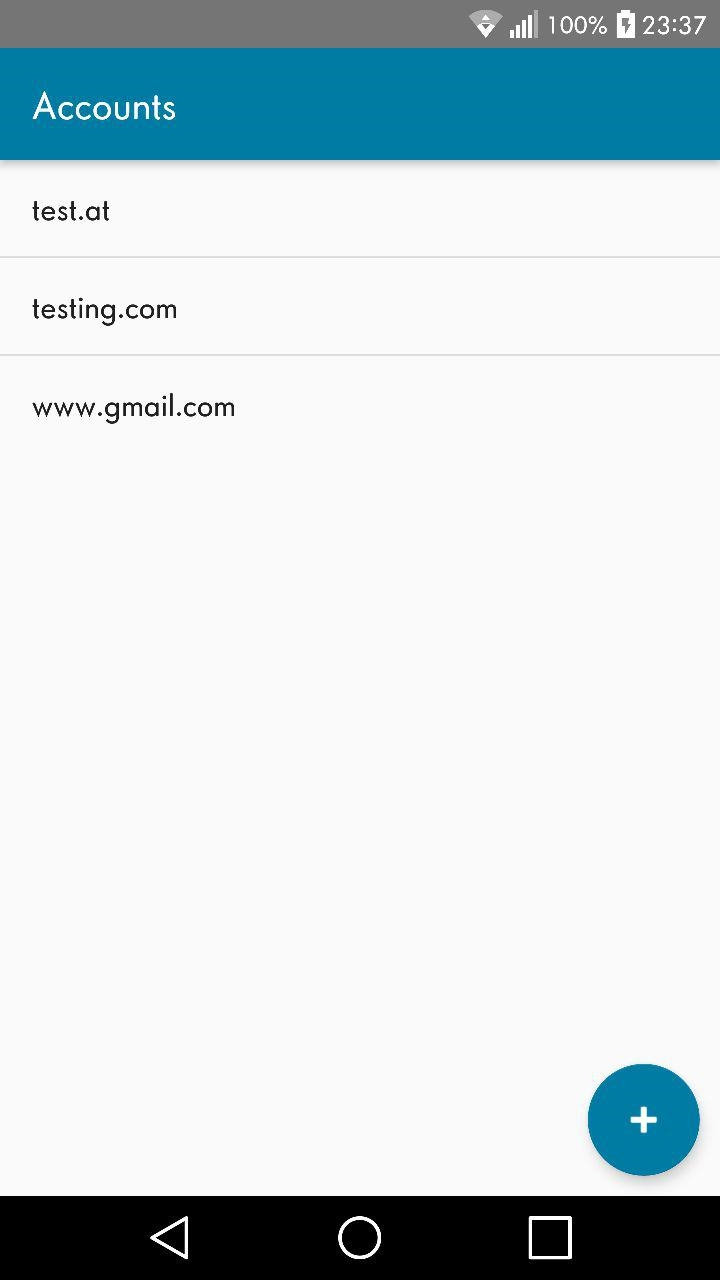
\includegraphics[width=3.5cm]{images/ShowAccountsActivity}\label{show_acc} }}
\qquad
\subfloat[]{{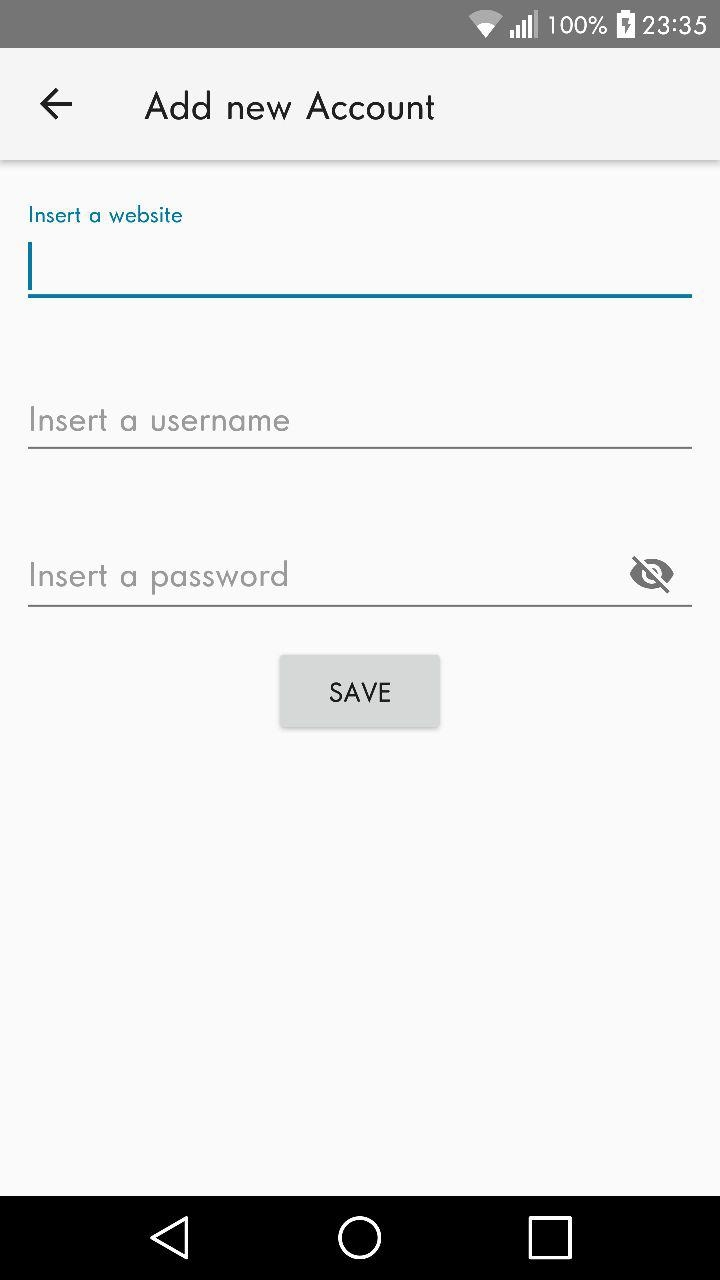
\includegraphics[width=3.5cm]{images/AddAccountActivity}\label{add_acc} }}
\qquad
\subfloat[]{{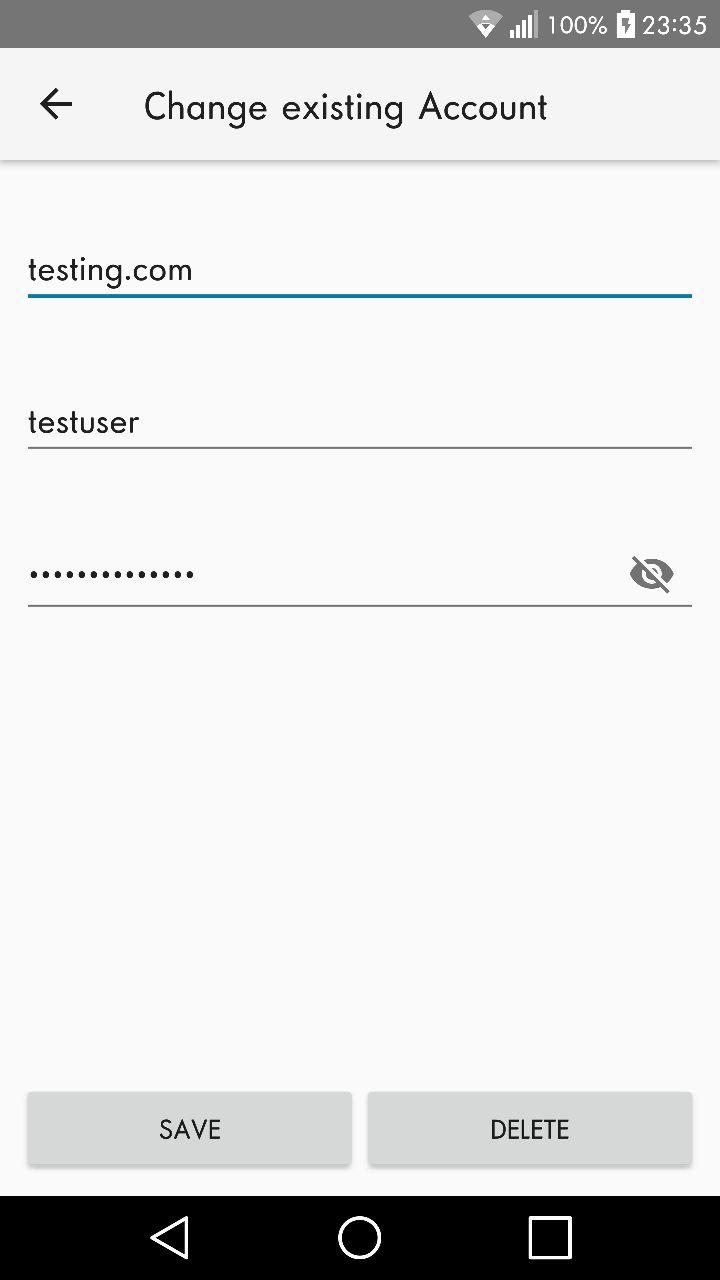
\includegraphics[width=3.5cm]{images/ChangeAccountActivity}\label{change_acc} }}
\qquad
\subfloat[]{{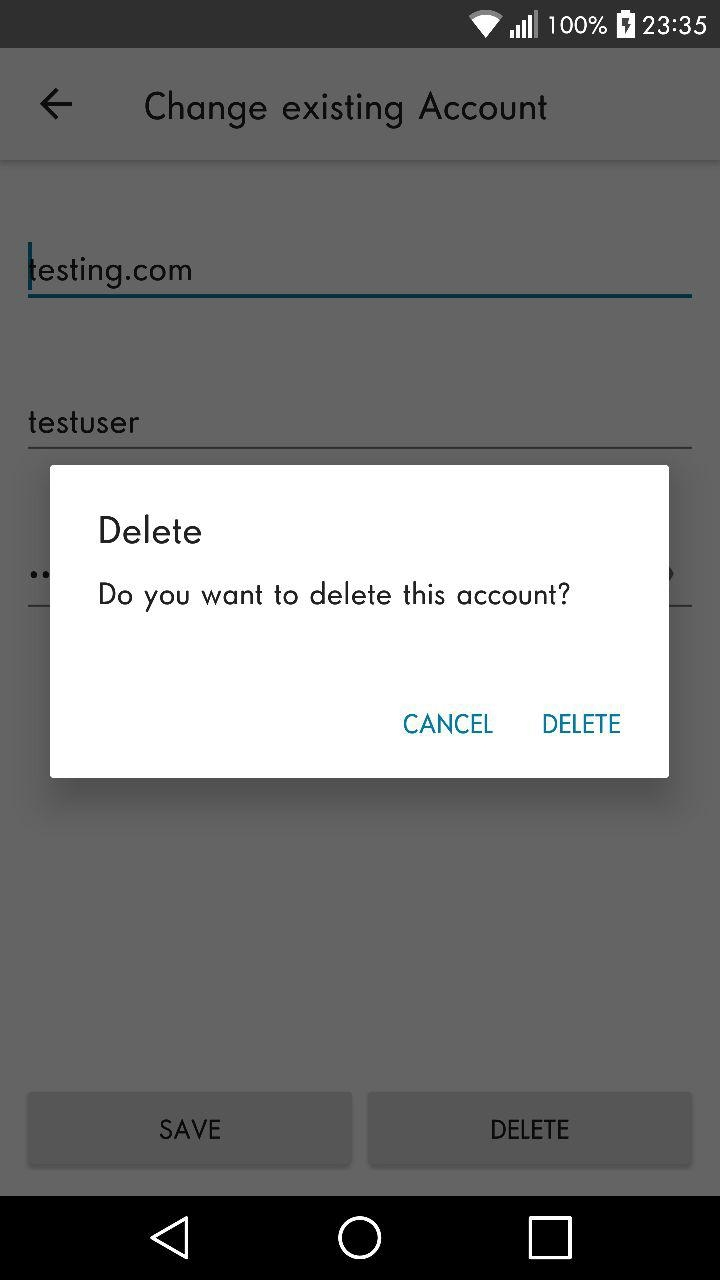
\includegraphics[width=3.5cm]{images/DeleteAccount}\label{prompt_delete} }}
\caption[Activity for managing Accounts]{Activity for managing Accounts; \protect\subref{show_acc}: listed accounts are shown. \protect\subref{add_acc}: interface where the user can add accounts. \protect\subref{change_acc}: the user can change selected account. \protect\subref{prompt_delete}: user is asked before deleting credentials.}
\label{fig:accountactivity}
\end{figure}

%-------------------------------------------------------------------------------------

\subsection{Activity for Bluetooth Connection}
After selecting the menu item \textit{Connection}, the app checks immediately if Bluetooth is enabled. If it is not turned on, the user is asked via prompt to enable Bluetooth. (Figure \ref{fig:connectionactivity}\protect\subref{prompt_bt}
If the activation is denied, the application will return to the main activity with an error message displayed in Figure \ref{fig:connectionactivity}\protect\subref{bt_notEnabled}. \\
Once Bluetooth is enabled, the accounts available for sharing are listed. At first, the application does not advertise any data. The user is asked to select an account to send to the Web Bluetooth API. (Figure \ref{fig:connectionactivity}\protect\subref{not_advertising}) Before any credentials are shared, the user is asked to authenticate himself. This is done by scanning his fingerprint or entering his master password. Figure \ref{fig:connectionactivity}\protect\subref{advertising} shows that only after successful authentication the advertising starts.

\begin{figure}[H]
\centering
\subfloat[]{{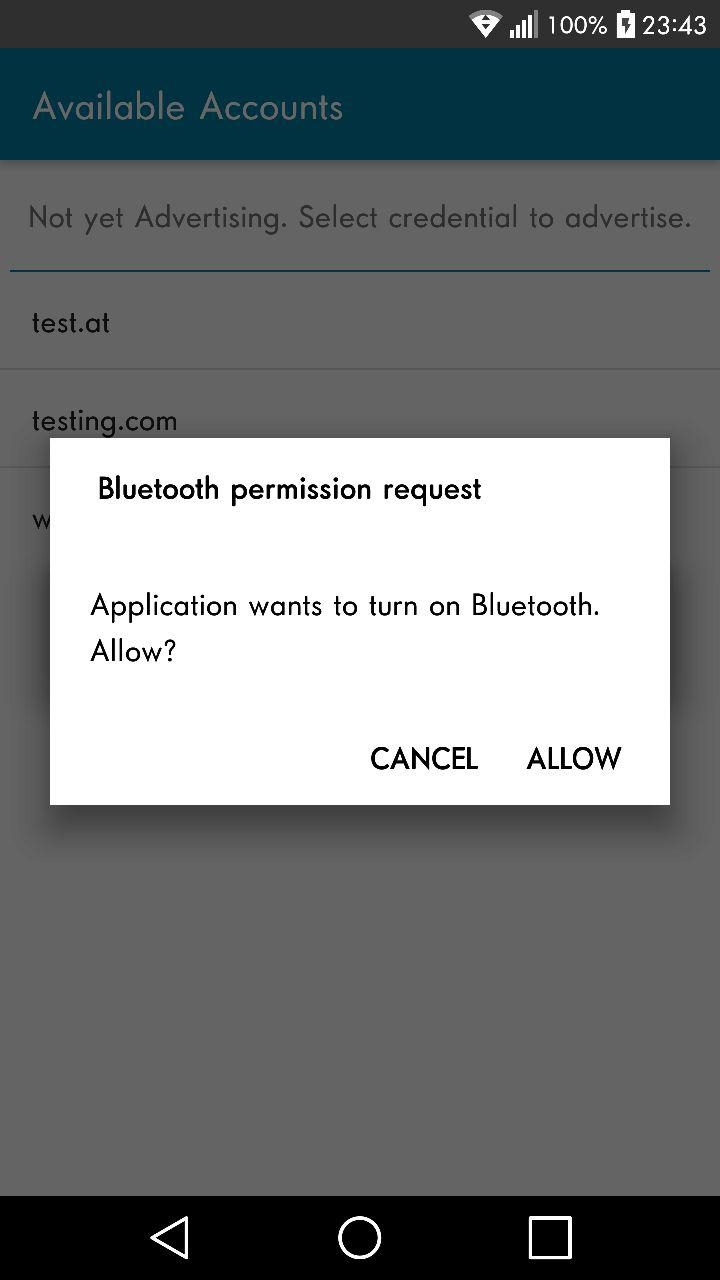
\includegraphics[width=3.5cm]{images/BT_english}\label{prompt_bt} }}
\qquad
\subfloat[]{{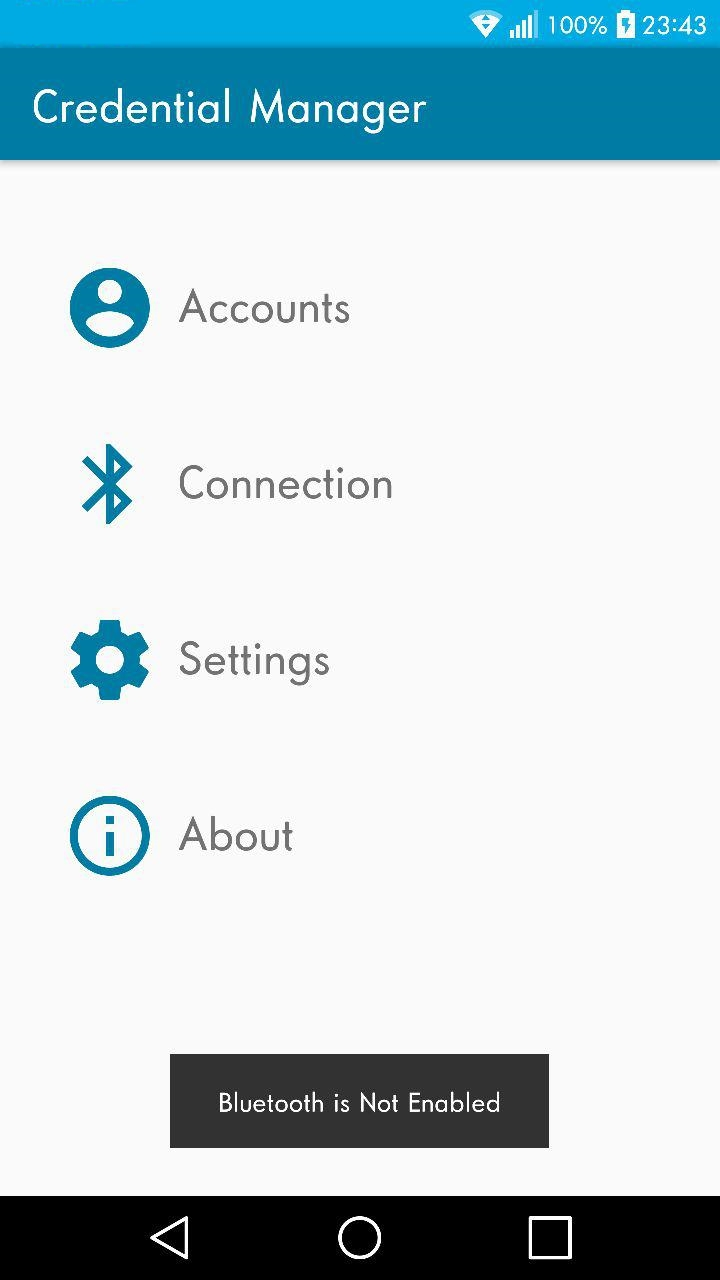
\includegraphics[width=3.5cm]{images/BTNotEnabled}\label{bt_notEnabled} }}
\qquad
\subfloat[]{{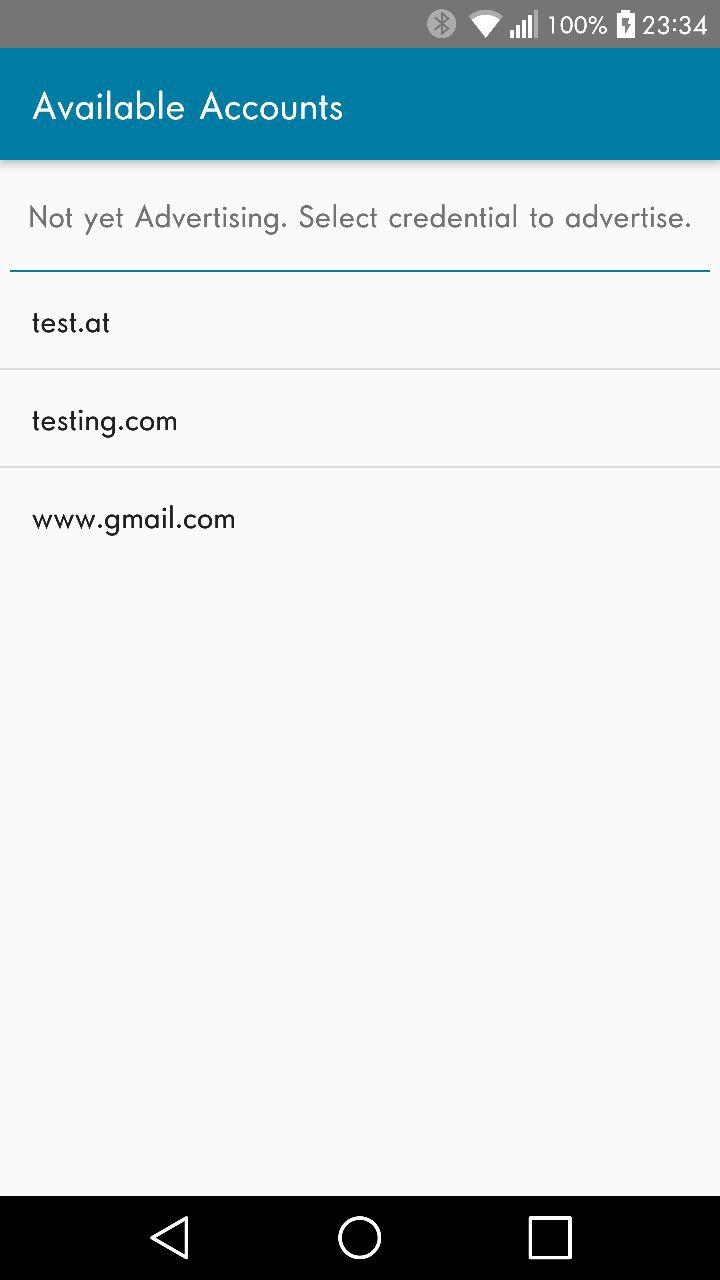
\includegraphics[width=3.5cm]{images/AvailableAccounts}\label{not_advertising} }}
\qquad
% !!!!!!!!!!!!! change jpg once programming done and working!
\subfloat[]{{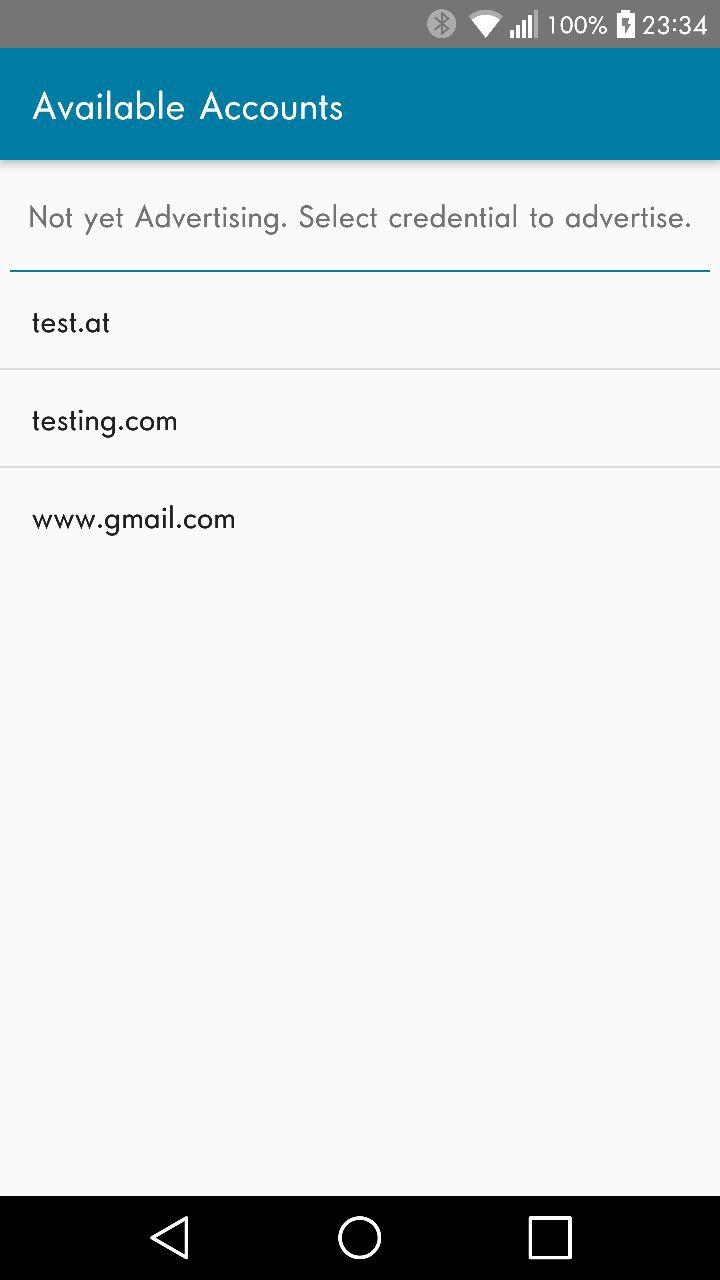
\includegraphics[width=3.5cm]{images/AvailableAccounts}\label{advertising} }}
%\qquad
%\subfloat[Asking the user before deleting the credential out of the database]{{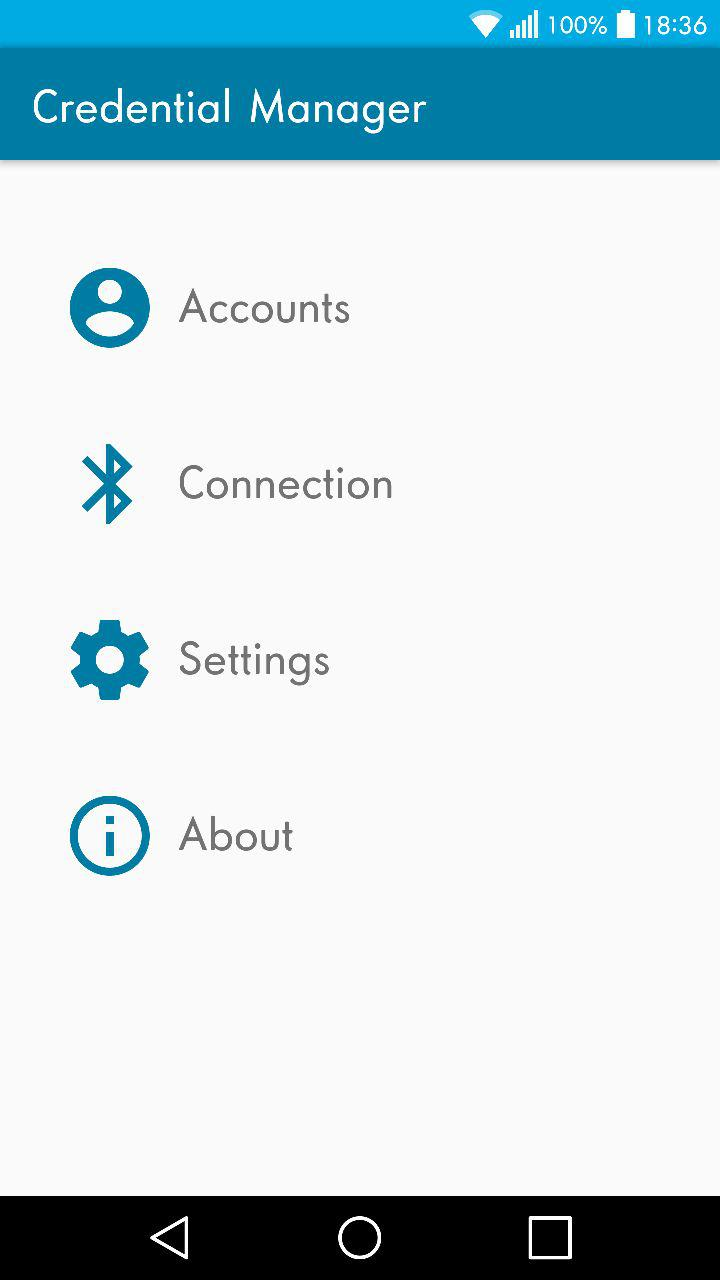
\includegraphics[width=5cm]{images/MainActivity} }}
\caption[Activity for Bluetooth Connection]{Activity for Bluetooth Connection; \protect\subref{prompt_bt}: a prompt is shown to the user to enable Bluetooth. \protect\subref{not_advertising}: is shown when the application is not advertising. \protect\subref{advertising}: is shown after user selected a credential to send.}
\label{fig:connectionactivity}
\end{figure}

%-------------------------------------------------------------------------------------


\subsection{Storage using greenDao ORM}
Since one goal is to store user credentials on the phone, we need a suitable database structure. One option was a common SQLite database. SQLite databases use SQL queries to store, retrieve and delete data. However, SQL queries can be vulnerable to security attacks, for example, second-order SQL injections. As stated in \cite{katole2018detection} a SQL injection is defined as a method where code is injected. This exploits a security vulnerability in the database layer of an application. It is done by modifying input data which then alters the SQL query. This procedure increases the risk of storing data unsafely and may lead to a vulnerable application. \cite{katole2018detection} also states that the risk of a SQL injection attack can increase due to not investing sufficient development time or lack of experience. We decided not to implement traditional SQL queries.

For this project, we use an object/relational mapping. It manages the tasks of storing, deleting, updating and querying. We decided on the greenDAO ORM \cite{Greendao} as it has an overall good performance. Additionally, it does not require as much programming effort compared to other frameworks as discussed in \cite{DBLP:conf/mascots/PuST16}. \\
Before setting up the database, we included the greenDAO plugin. To set up the database, a DaoMaster had to be initialized. The DaoMaster is provided from the helper class \texttt{DevOpenHelper}, and handles the database set up and creates DaoSessions. Listing \ref{lst:db_master} shows this process.

\begin{lstlisting}[caption=Creation of database, label=lst:db_master]
DaoMaster.DevOpenHelper helper = 
        new DaoMaster.DevOpenHelper(this,"credentials-db");
Database db = helper.getWritableDb();
daoSession = new DaoMaster(db).newSession();
\end{lstlisting}
\vspace{0.5cm}

A DaoSession, on the other hand, manages the DAO object. It is an entity that we store into the database. DAO objects are created from a Java class. To define a Java class as a database-backed entity, annotations to the class-header and to the class members must be added. The class members define the columns of the database. Afterward, the greenDAO generator automatically generates all required methods. After this process is done, instances of the class can be stored into the greenDAO database. \cite{Greendao}

\subsubsection*{Load, insert and delete a database entry}
As mentioned before, the DaoSession manages DAO objects and they, in turn, handle all operations of the database. With the start of the application, the database is opened, and a new DaoSession is instantiated. To manage all interactions of DAO objects, we defined a database helper class. \\
Listing \ref{lst:db_insert} shows an example of how one credential is inserted into the database. The DaoSession calls the DAO object, and the object handles the insert method to store data into the database. The load and delete methods use the DaoSession as well. 

\begin{lstlisting}[caption= Insert entry into database, label=lst:db_insert]
public void insertNewAccount(Account account) {
    AccountDao accountDao = this.daoSession.getAccountDao();
    accountDao.insert(account);
}
\end{lstlisting}
\vspace{0.5cm}

The database created by the application lies on presistent memory of the mobile device, and can only be accessed from our app. In case of an attack even if the database content is dumped, the attacker if left with the encrypted data. In section \ref{arch_encryption} we discuss how data is encrypted before inserting into the database and decrypted again when fetching from it. \\

%-------------------------------------------------------------------------------------

\subsection{Encryption of Data}\label{arch_encryption}
%explaining the en and decryption of data, all about choosing a key: all about cipher and algorithm, code lines and android developer cites, modes paddings usw.
For en- and decryption of sensitive data there exist different possibilities. One option of storing passwords is hashing and storing the hash in the database. SHA256 or SHA512 are some hash algorithms as mentioned in \cite{ertaul2016implementation}. By hashing data for encryption, data can be recovered by multiple different attacks such as Brute Force or Dictionary attack. \\
Another way to store sensitive data is to hash it with a random string of bits, called \textit{salt}. It is stored with the hash of the plaintext. This can also become vulnerable to the Dictionary Attack as stated in \cite{3wrongways}. \\
Nowadays it is common to use a key derivation function to safely store passwords. They must generate a strong key that is secure against attacks. Latest key derivation functions are \textit{password-based key derivation function 2 (PBKDF2)}, \textit{Bcrypt}, and \textit{Scrypt}. As mentioned in \cite{ertaul2016implementation}, their security is strong.
However, PBKDF2 requires the user's input to generate the key for encryption. The generated key will depend on the password chosen by the user. \cite{Agilebits} As a result of the study conducted in \cite{DBLP:journals/ieeesp/YanBAG04}, users create passwords that may not be safe. In case of a very simple password, PBKDF2 cannot perform as securely as with a strong one. \cite{3wrongways}

Therefore, our goal is to provide safe en- and decryption without depending on the user's input. Also, all encryption takes place within the mobile phone, and there is no need for any public encryption component. Therefore, encryption and decryption can be done with the same key. \cite{DBLP:journals/ijnsec/ElminaamKH10} \\
We decided to encrypt data using the AES algorithm. We used the Galois/Counter Mode (GCM) as our cipher mode. GCM uses the Counter Mode (CTR) internally. \cite{AESJavaAndroid} A counter value for each block is encrypted and only uses as many bits as required from the last block. Hence, it turns the block cipher into a stream cipher, and no padding is required. \cite{IVtransmission} \\
We instantiated the cipher, as seen in Listing \ref{lst:cipher}.

\begin{lstlisting} [caption=Instantiation of cipher, label=lst:cipher]
final Cipher cipher = Cipher.getInstance("AES/GCM/NoPadding");
\end{lstlisting}

The GCM provides confidentiality, integrity, and authenticity for securing data. \cite{AESJavaAndroid} Hence, it is ideal for generating a secret key that is also independent of user data. For encryption, GCM takes as input the IV, a plaintext, and additional authenticated data (AAD). The AAD is not required and does not affect the security of the GCM mode. \cite{AADsecure} \\
In this project, we passed the plaintext and the IV. The output of encryption is the ciphertext and an authentication tag. \cite{dworkin2007sp} The authentication tag contains information, that is associated with the data encrypted. It is useful in case of unauthorized change to the encrypted data. \cite{AESJavaAndroid} When decrypting data, GCM expects the IV, a ciphertext, the authentication tag, and the AAD, if it has been passed during encryption. Only if the authentication tag calculated during encryption and then passed one are identical, the plaintext is returned. \cite{dworkin2007sp}

Important for the Android implementation of GCM is the length of the initialization vector (IV). National Institute of Standards and Technology recommends 96 bits for the IV to be fast and secure. \cite{dworkin2007sp} To ensure that a unique IV is used with every encryption, a new one is generated upon each call of the encrypt method. Afterward, we concatenate the IV to the ciphertext. Before decryption, the IV is separated from the ciphertext again. We created the IV using the strong random number generator \textit{SecureRandom} from the Android Library. \cite{SecureRandom}

A problem occurred when calling the method \texttt{cipher.doFinal(cipherText)} while using the SecureRandom class to generate our IV. Android insists on using their default method \texttt{cipher.getIV();} for generating the IV. \cite{DefaultIV} argues that using that IV may not be secure because the risk of reusage is given. Reusing an IV results in a vulnerable implementation and compromises the security of data. The IV being unique is almost as important as the key being secret. \cite{dworkin2007sp} \\
Therefore, we decided to provide the IV by a SecureRandom instead of using the default method. Android believes we may be working unsafely, because we are not using the provided method \texttt{cipher.getIV()}. To solve the problem, we set the \textit{setRandomizedEncryptionRequired()} property to \textit{false} when we generated the key, which is shown in Listing \ref{lst:key}. This way Android allows using our generated IV. \cite{SecretsInAndroid}

\begin{lstlisting} [caption=Setting properties of secret key, label=lst:key]
SpecBuilder.setKeySize(128)
    .setBlockModes(KeyProperties.BLOCK_MODE_GCM)
    .setEncryptionPaddings(KeyProperties.ENCRYPTION_PADDING_NONE)
    .setRandomizedEncryptionRequired(false);
\end{lstlisting}

After generation of the key and successful encryption, it is crucial to store the key securely. We rely on the Android Keystore for this task. Chapter \ref{arch_keystore} discusses the safe storage of the key. \\


%maybe put pieces of console to show what is effectivly store into the data base and how it is retrieved and decrypted again?

%-------------------------------------------------------------------------------------

\subsection{Secure Storage of Secret Key} \label{arch_keystore}
%explaining what it done with the key afterwards, after creation, how can it be safely stored and not revealed, tee never leaves phone and if then it is destroyed, attacker is only left with encrypted dump of DB, without key cannot retrieve plaintext; what is the tee, where is it, how is it managed and is it on every phone? which phones?
As stated in \cite{dworkin2007sp} and \cite{DBLP:conf/ccs/CooijmansRP14},  in practice the secrecy of the key and secure storage are crucial. If the key can be retrieved from the device, the data's security is exceedingly compromised. With the key, all ciphertexts can be decrypted easily. Therefore, we need a system to ensure safe storage of the key.

The \textit{AndroidKeystore} system allows safe storage of cryptographic keys. Applications use this Android Framework API  to access Keystore functionality. \cite{HWBKeyStore} The AndroidKeystore lets an app store and manage its credentials while making sure no other application can access them. \cite{AndroidKeyStoreSystem}

To increase the security of the key, we made use of the hardware-based security feature provided by a specific realization of the AndroidKeystore. Modern mobile phones' processors are equipped with ARM TrustZone Technology. \cite{DBLP:conf/ccs/CooijmansRP14} This technology separates the hardware into two operations systems (OS): a secure world OS and normal OS. The secure world OS is also known as a \textit{Trusted Execution Environment} (TEE). The TEE ensures that data does not get leaked out of this trusted environment. Hence, keys stored in the TEE cannot be retrieved. Utilization of the TEE depends on the device manufacture. On devices equipped with a Qualcomm processor with TrustZone Technology, the AndroidKeystore is automatically stored in the TEE. \cite{DBLP:conf/ccs/CooijmansRP14} This represents the most secure option to store keys. \cite{SecureDataEncryption} If TEE is not supported, the keys are stored in a system provided emulated software environment. However, keys will be removed when deleting the application that created them.

Before we can generate a key or use it for encryption, we must instantiate and load the Keystore.
A key is stored into the Keystore under a given identifier, also known as \textit{alias}. \cite{DBLP:conf/ccs/CooijmansRP14} The alias is a string that defines a reference to the key. All cryptographic operations are done in the background, and key material is never exposed. Hence, the alias is needed everytime data is en- and decrypted. \\
Also, the lock screen must be set in order to reference the key. The KeyguardManager is used for this process. The method \texttt{isDeviceSecure()} returns if the device is secured with a PIN, pattern or password. If the device is not locked, the AndroidKeystore is not instantiated, and cryptographic calculations cannot take place. \\



%-------------------------------------------------------------------------------------

\subsection{Authentication through Biometrics}
To securely protect user credentials, the app uses biometric authentication. As biometric authentication, we use the user's fingerprint. Whenever the user wants to access or send credentials, the application requires fingerprint authentication from the user.

Before the actual authentication can take place, the application checks some requirements. For this process, an instance of the Android class \textit{FingerprintManager} is required. The class handles accesses to the fingerprint hardware. \cite{FingerprintManager} \\
Firstly, the application checks if a fingerprint sensor is available. The method \texttt{isHardwareDetected()} is called on the FingerprintManager to ensure the device supports fingerprint scanning.  If the phone does not have a fingerprint sensor, the user has the option of entering a master password. \\
The next requirement is the permission to use fingerprint scanning. This must be granted by the Android permission system, which is discussed in Section \ref{limitations_root}. \\
Also, the user must have at least one fingerprint registered on the device. \cite{Techotopia} The FingerprintManager uses the method \texttt{hasEnrolledFingerprints()} to check this. If no fingerprints are saved, a message is displayed as shown in Figure \ref{fig:authentication}\protect\subref{auth_none}. \\
Before starting authentication via fingerprint, the application makes sure the lock screen is secured. This is done with the Android class \texttt{KeyguardManager}. \cite{KeyguardManager} The KeyguardManager provides access to the lock screen and checks if a PIN, password, pattern is set or if the SIM card is locked. The mobile device must be secured for the authentication process to proceed.
%technical stuff: keystore, key, cipher, authenticate(); or insert code listing to see how cipher of fingerprint is created??

As mentioned above, upon every request to send an account login the user has to re-authenticate. This security mechanism would prohibit unintentional distribution of sensitive data. Therefore, the security would not be compromised if the user left their phone unattended with the application still running. \\

\begin{figure}[H]
\centering
\subfloat[]{{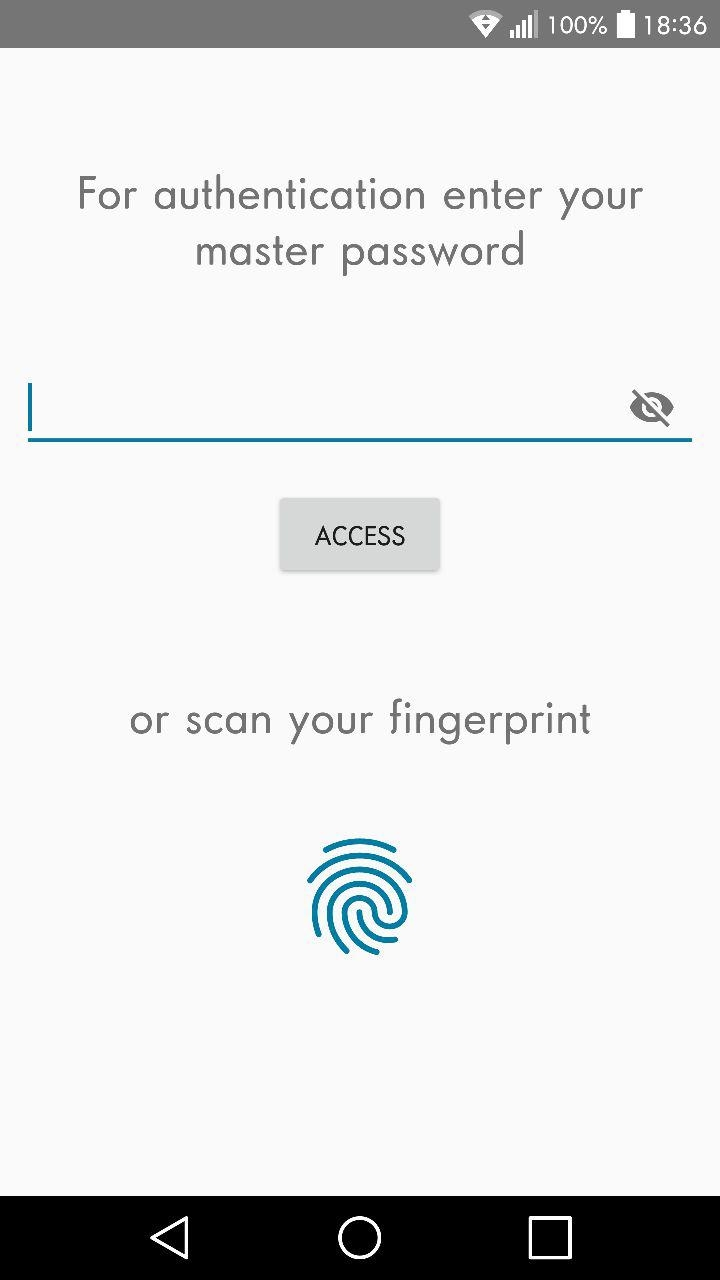
\includegraphics[width=3.5cm]{images/AuthenticationScreen}\label{auth_screen} }}
\qquad
\subfloat[]{{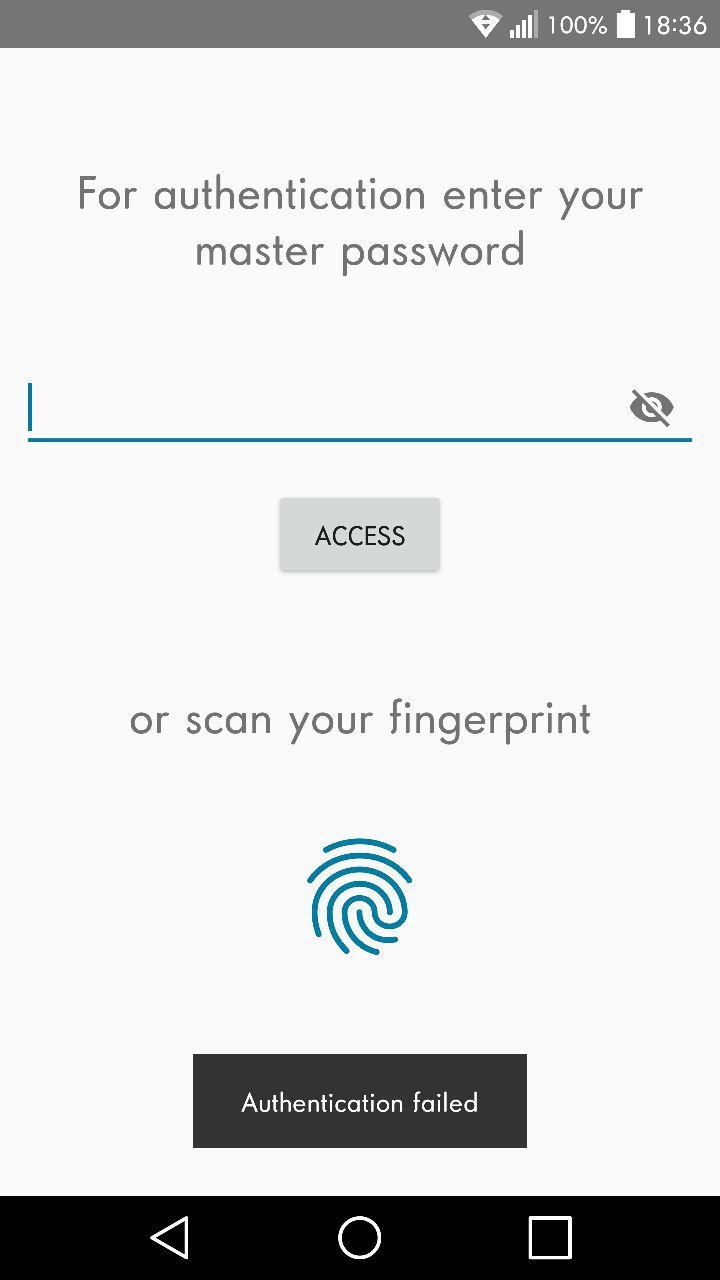
\includegraphics[width=3.5cm]{images/AuthenticationFailed}\label{auth_fail} }}
\qquad
\subfloat[]{{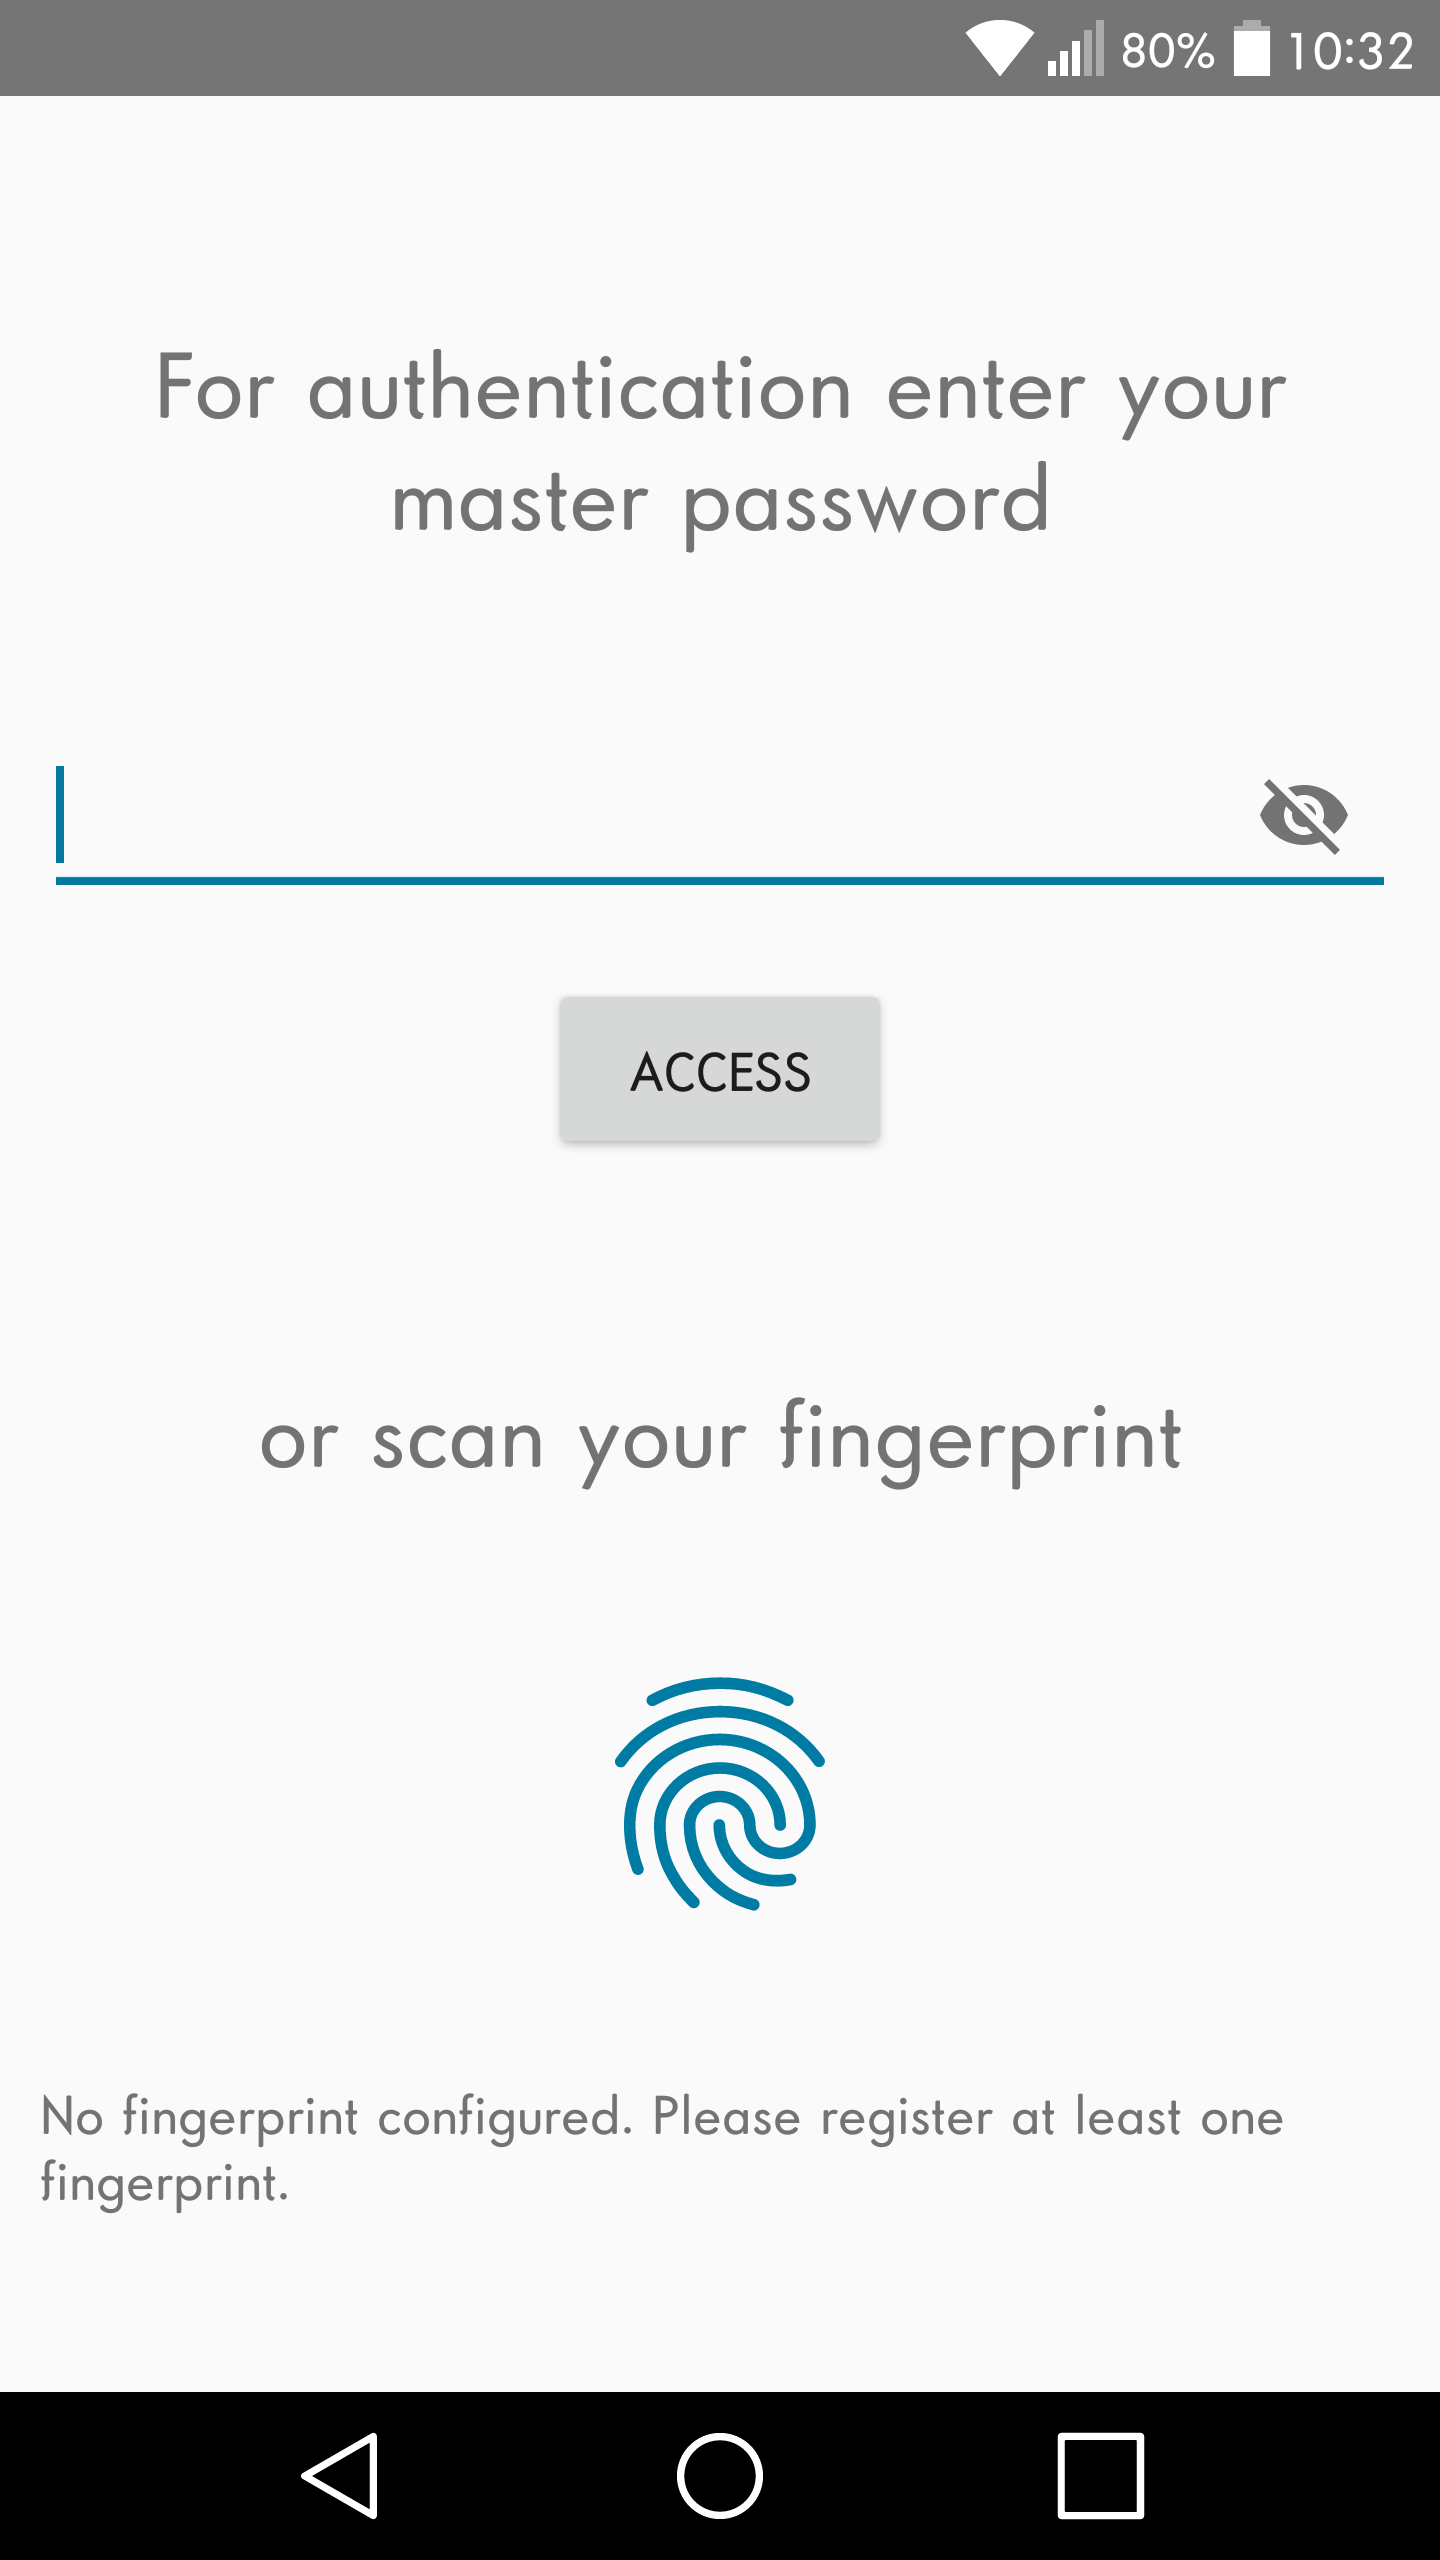
\includegraphics[width=3.5cm]{images/fingerprint_noneRegistered}\label{auth_none} }}
\caption[Activity for Authentication]{Activity for Authentication; \protect\subref{auth_screen}: the user is asked to auhenticate themselves. \protect\subref{auth_fail}: authentication failes if incorrect fingerprint is scanned. \protect\subref{auth_none}: is shown if no fingerprints are registered on the device.}
\label{fig:authentication}
\end{figure}

%-------------------------------------------------------------------------------------

\subsection{Chrome Extension with the Web Bluetooth API}
After discussing in depth the credential storage, encryption, and the authentication, we will briefly describe the communication of the extension and the Android application.

Additionally to the application, we implemented an extension for the Chrome browser. Chrome has an API, Web Bluetooth API, to support a BLE connection. \cite{WebBTAPI} This makes it possible for a website to communicate with a near BLE device. The BLE device advertises characteristics, and the Web Bluetooth API reads them. Our BLE device is the application, and the extension implements the API. \\
The workflow is as follows: firstly, the application advertises a specific service containing the credentials. Services are specified by a UUID and can advertise characteristics and descriptors. To distinguish our custom service from the other BLE services we defined a UUID in the code. The extension will only connect to the service that matches the defined UUID. Once found, the connection of the Bluetooth devices takes place. Only after the devices have been paired, the Web Bluetooth API can read the characteristics. Every characteristic has a UUID of its own. This helps to distinguish them easily. We defined the username and password as our characteristics. They are retrieved from the service with the method \texttt{service.getCharacteristic();}. To read the values, the Web Bluetooth API uses the method \texttt{characteristic.readValue();}. \cite{WebBTAPI}

Usually, the Android application has the central role in a Bluetooth Low Energy (BLE) connection. When communicating with a BLE device, such as a heart rate monitor, the BLE device has the peripheral role. The app serves as the client and the BLE device as the server, sending data that the application wants to receive. \\
In this scenario, however, the roles are reversed. The Android app serves as the server. It advertises data that the extension wants to read. Consequently, the application opens a GATT server to advertise the characteristics. The extension, on the other hand, acts as the client and implements a GATT service to retrieve the characteristics. The extension reads the values and fills them into the login fields. \\